\documentclass{article}

\usepackage[margin=0.5in]{geometry}
\usepackage{enumitem}
\usepackage{graphicx}

\usepackage[group-separator={,}]{siunitx}

\title{2.3 Combinatorics Homework Problems}
\author{}
\date{}

\begin{document}
\maketitle

\begin{enumerate}
    \item In how many ways can the letters $A$, $B$, $C$, and $D$ be arranged so that no letter is adjacent to any letter that comes immediately before it or immediately after it alphabetically?
        \vspace{3cm}
    \item Professor Zhang has nine different language books lined up on a bookshelf: two Arabic, three German, and four Spanish.
        How many ways are there to arrange the nine books on the shelf keeping the Arabic books together and keeping the Spanish books together?
        \vspace{3cm}
    \item If there are $3$ boys and $4$ girls in a group and two are chosen to give a report, what is the probability that one boy and one girl are chosen?
        \vspace{3cm}
    \item A game board consists of $64$ squares that alternate in color between black and white.
        The figure below shows square $P$ in the bottom row and square $Q$ in the top row.
        A marker is placed at $P$.
        A step consists of moving the marker onto one of the adjoining white squares in the row above.
        How many $7$-step paths are there from $P$ to $Q$?
        (The figure shows a sample path.)
        \begin{center}
            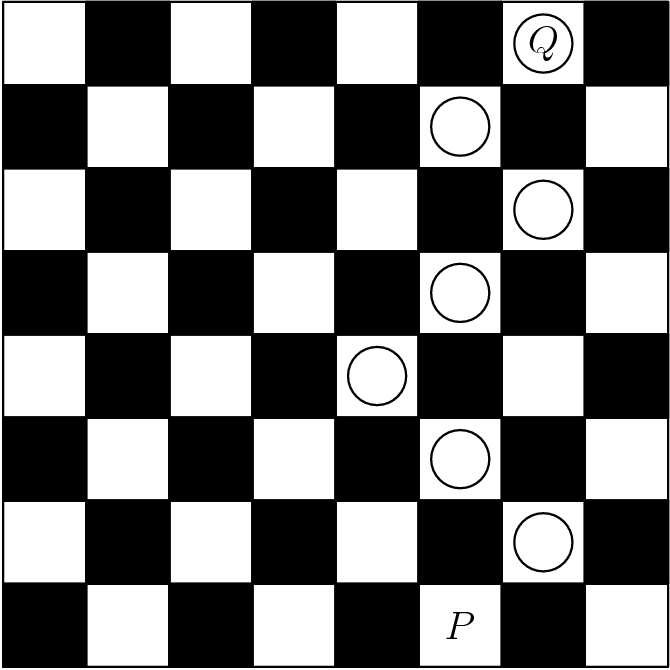
\includegraphics[scale=0.25]{checker-board.png}
        \end{center}
        \vspace{3cm}
\end{enumerate}

\end{document}
